\section*{7. Case Studies}

To evaluate the effectiveness of PipeViz, we conducted multiple case studies exploring how compiler optimizations and LLM-guided transformations affect pipeline execution behavior. These studies focus on analyzing hazard frequency, instruction scheduling efficiency, memory access patterns, and instruction-level parallelism across different execution models. By combining cycle-accurate simulation with contextual LLM analysis, the experiments demonstrate how PipeViz can be used both as an educational visualization platform and as a practical micro-architectural optimization tool.

The case studies specifically investigate two optimization scenarios: cache-aware matrix multiplication and compiler-assisted loop unrolling. In each experiment, the system compares baseline implementations against optimized variants while visualizing the resulting changes in hazard behavior, pipeline stalls, and execution overlap. These experiments highlight the relationship between high-level algorithmic transformations and low-level processor execution characteristics.

\subsection*{Case Study 1. LLM-Driven Cache Optimization and Pipeline Analysis for Matrix Multiplication}

\textbf{Methodology and Experimental Setup.} This case study demonstrates the integration of LLM-assisted code optimization with detailed micro-architectural pipeline simulation using the PipeViz tool. A baseline matrix multiplication implementation (\texttt{64$\times$64} double-precision matrices) was submitted to the pipeline visualization system configured with a static in-order execution model targeting \texttt{AArch64} architecture. The original code employed a triple-nested loop structure (\texttt{i-j-k} ordering) with no explicit cache optimization. Here is the User code input:

\begin{lstlisting}[language=C, basicstyle=\ttfamily\scriptsize, tabsize=2]
#include <stdio.h>
#include <stdlib.h>
#include <string.h>
#include <time.h>

#define N 64      // Matrix size
#define B 8       // Blocking factor (cache line size consideration)

void matrix_multiply(double x[N][N], double y[N][N], double z[N][N]) {
    for (int i = 0; i < N; i++) {
        for (int j = 0; j < N; j++) {
            for (int k = 0; k < N; k++) {
                x[i][j] = x[i][j] + y[i][k] * z[k][j];
            }
        }
    }
}

// Initialize matrices
void init_matrices(double x[N][N], double y[N][N], double z[N][N]) {
    for (int i = 0; i < N; i++) {
        for (int j = 0; j < N; j++) {
            x[i][j] = 0.0;
            y[i][j] = (double)(i * N + j);
            z[i][j] = (double)((i + j) % N);
        }
    }
}

int main() {
    double (*x)[N] = malloc(sizeof(double) * N * N);
    double (*y)[N] = malloc(sizeof(double) * N * N);
    double (*z)[N] = malloc(sizeof(double) * N * N);
    
    if (!x || !y || !z) {
        fprintf(stderr, "Memory allocation failed\n");
        return 1;
    }

    init_matrices(x, y, z);
    
    // Run blocked version
    matrix_multiply(x, y, z);
    
    // Print result sample
    printf("Result[0][0] = %f\n", x[0][0]);
    printf("Result[5][5] = %f\n", x[5][5]);
    
    free(x);
    free(y);
    free(z);
    
    return 0;
}
\end{lstlisting}

After compilation with user-specified optimization flags, the generated assembly code was extracted and simulated through the five-stage pipeline (\texttt{IF}$\rightarrow$\texttt{ID}$\rightarrow$\texttt{EX}$\rightarrow$\texttt{MEM}$\rightarrow$\texttt{WB}), with the tool automatically identifying and visualizing data hazards (\texttt{RAW}, \texttt{WAR}, \texttt{WAW}) and structural hazards at each clock cycle. This baseline simulation established performance metrics, including pipeline stalls, bubble insertion patterns, and memory access characteristics that would serve as the comparison point for optimization. Here is the figure~\ref{fig:cycle-instructions} that shows the "\texttt{Static in order}" cycle-by-cycle instructions.

\begin{figure*}[t]
  \centering
  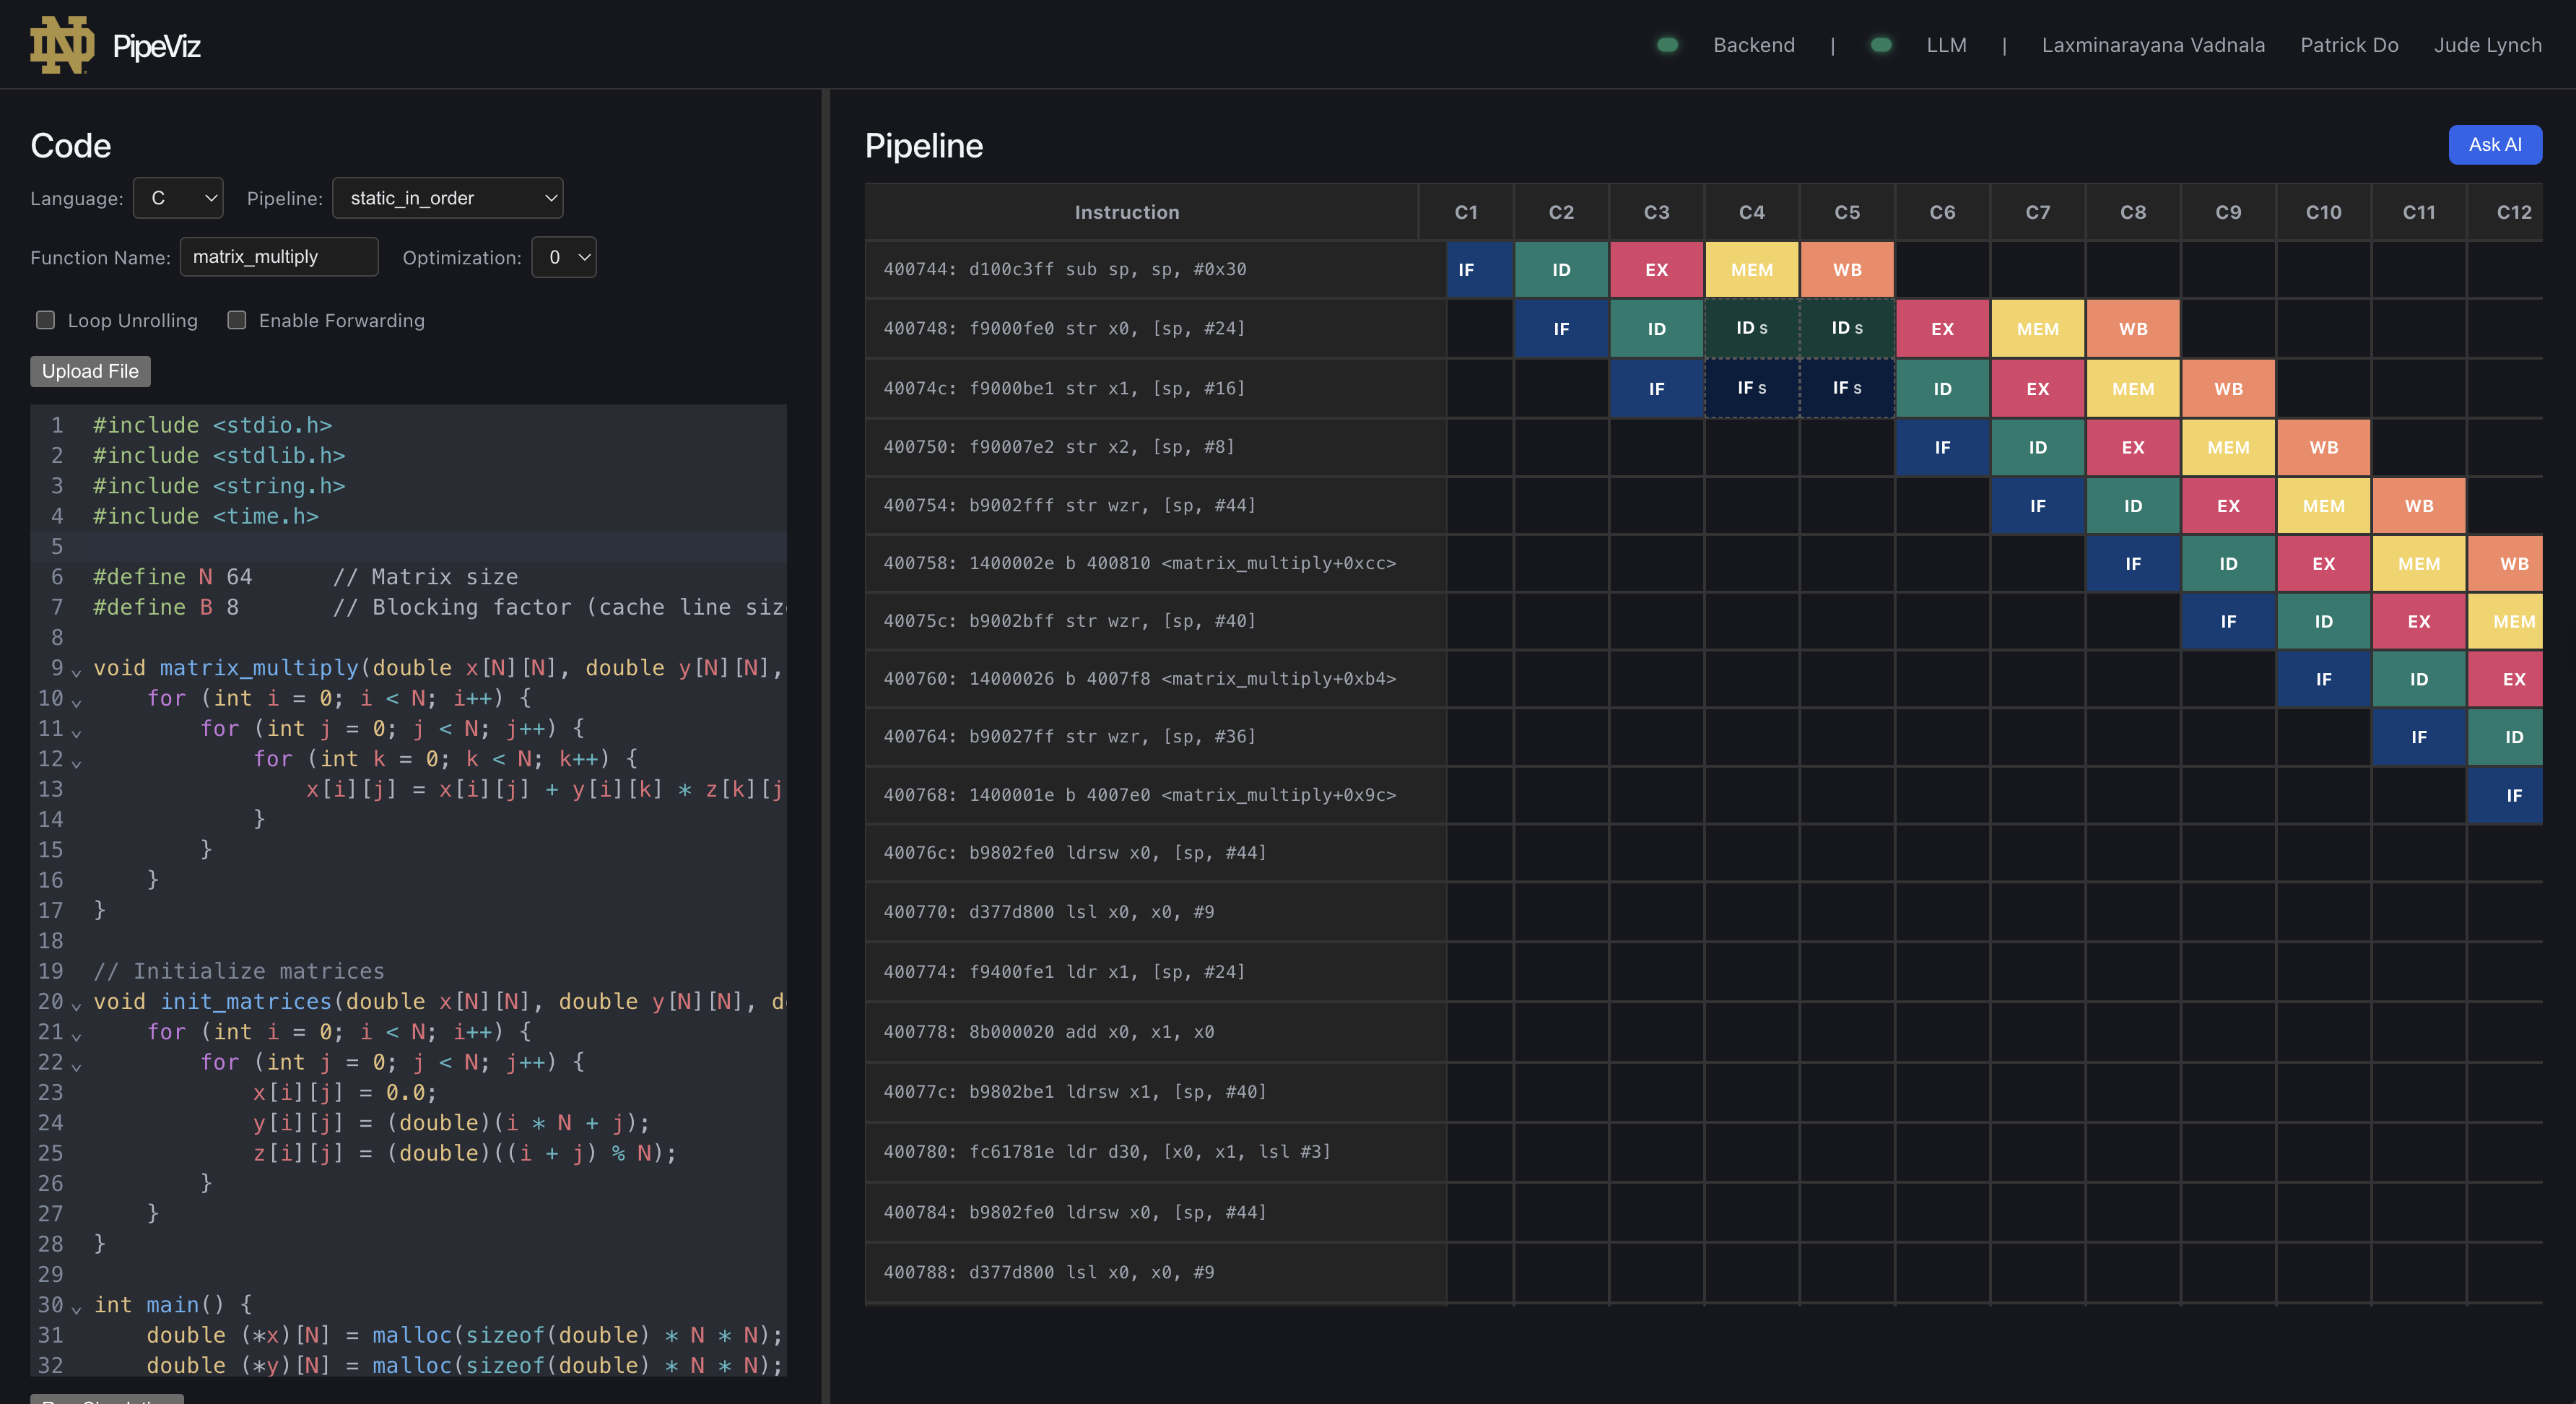
\includegraphics[width=\textwidth]{fig/cycle-instructions.png}
  \vspace{-0.25in}
  \caption{The PipeViz user interface showing the cycle-by-cycle instructions. This run refers to the matrix multiplication case study.}
  \label{fig:cycle-instructions}
\end{figure*}

\textbf{LLM-Suggested Optimization Strategy.} The integrated LLM-based chatbot was provided with the complete context of the baseline implementation—including the original C source code, generated \texttt{AArch64} assembly, and the detailed pipeline simulation data showing hazard patterns and execution bottlenecks. Analyzing this micro architectural feedback, the LLM proposed a cache-blocked (tiled) matrix multiplication algorithm using a blocking factor of \texttt{8} (matching the original \texttt{B} constant). The optimized implementation introduces an outer tile-iteration structure (\texttt{ii-jj-kk} loops) that partitions the matrix operations into \texttt{8$\times$8} subblocks, with inner loops (\texttt{i-j-k}) operating within each tile. Critically, the optimization accumulates partial results in a scalar temporary (\texttt{sum}) before writing back to the output matrix, reducing the number of load-modify-store operations per element. This restructuring aims to improve spatial and temporal locality, keeping working sets within \texttt{L1} cache boundaries and potentially reducing memory-stage stalls observed in the baseline pipeline simulation.

Here is the LLM suggested C code:

% \begin{lstlisting}[language=C, basicstyle=\footnotesize]
% #define N 64
% #define B 8

% void matrix_multiply(double x[N][N],
%                     double y[N][N],
%                     double z[N][N]) {

%     for (int ii = 0; ii < N; ii += B) {
%         for (int jj = 0; jj < N; jj += B) {
%             for (int kk = 0; kk < N; kk += B) {

%                 for (int i = ii; i < ii + B; i++) {

%                     for (int j = jj; j < jj + B; j++) {

%                         double sum = x[i][j];

%                         for (int k = kk; k < kk + B; k++) {
%                             sum += y[i][k] * z[k][j];
%                         }

%                         x[i][j] = sum;
%                     }
%                 }
%             }
%         }
%     }
% }
% \end{lstlisting}

\begin{lstlisting}[language=C, basicstyle=\ttfamily\scriptsize, tabsize=2]
#define N 64
#define B 8

void matrix_multiply(double x[N][N], double y[N][N], double z[N][N]) {
  for (int ii = 0; ii < N; ii += B) {
    for (int jj = 0; jj < N; jj += B) {
      for (int kk = 0; kk < N; kk += B) {
        for (int i = ii; i < ii + B; i++) {
          for (int j = jj; j < jj + B; j++) {
            double sum = x[i][j];
            for (int k = kk; k < kk + B; k++) {
              sum += y[i][k] * z[k][j];
            }
            x[i][j] = sum;
          }
        }
      }
    }
  }
}
\end{lstlisting}

\begin{figure*}[t]
  \centering
  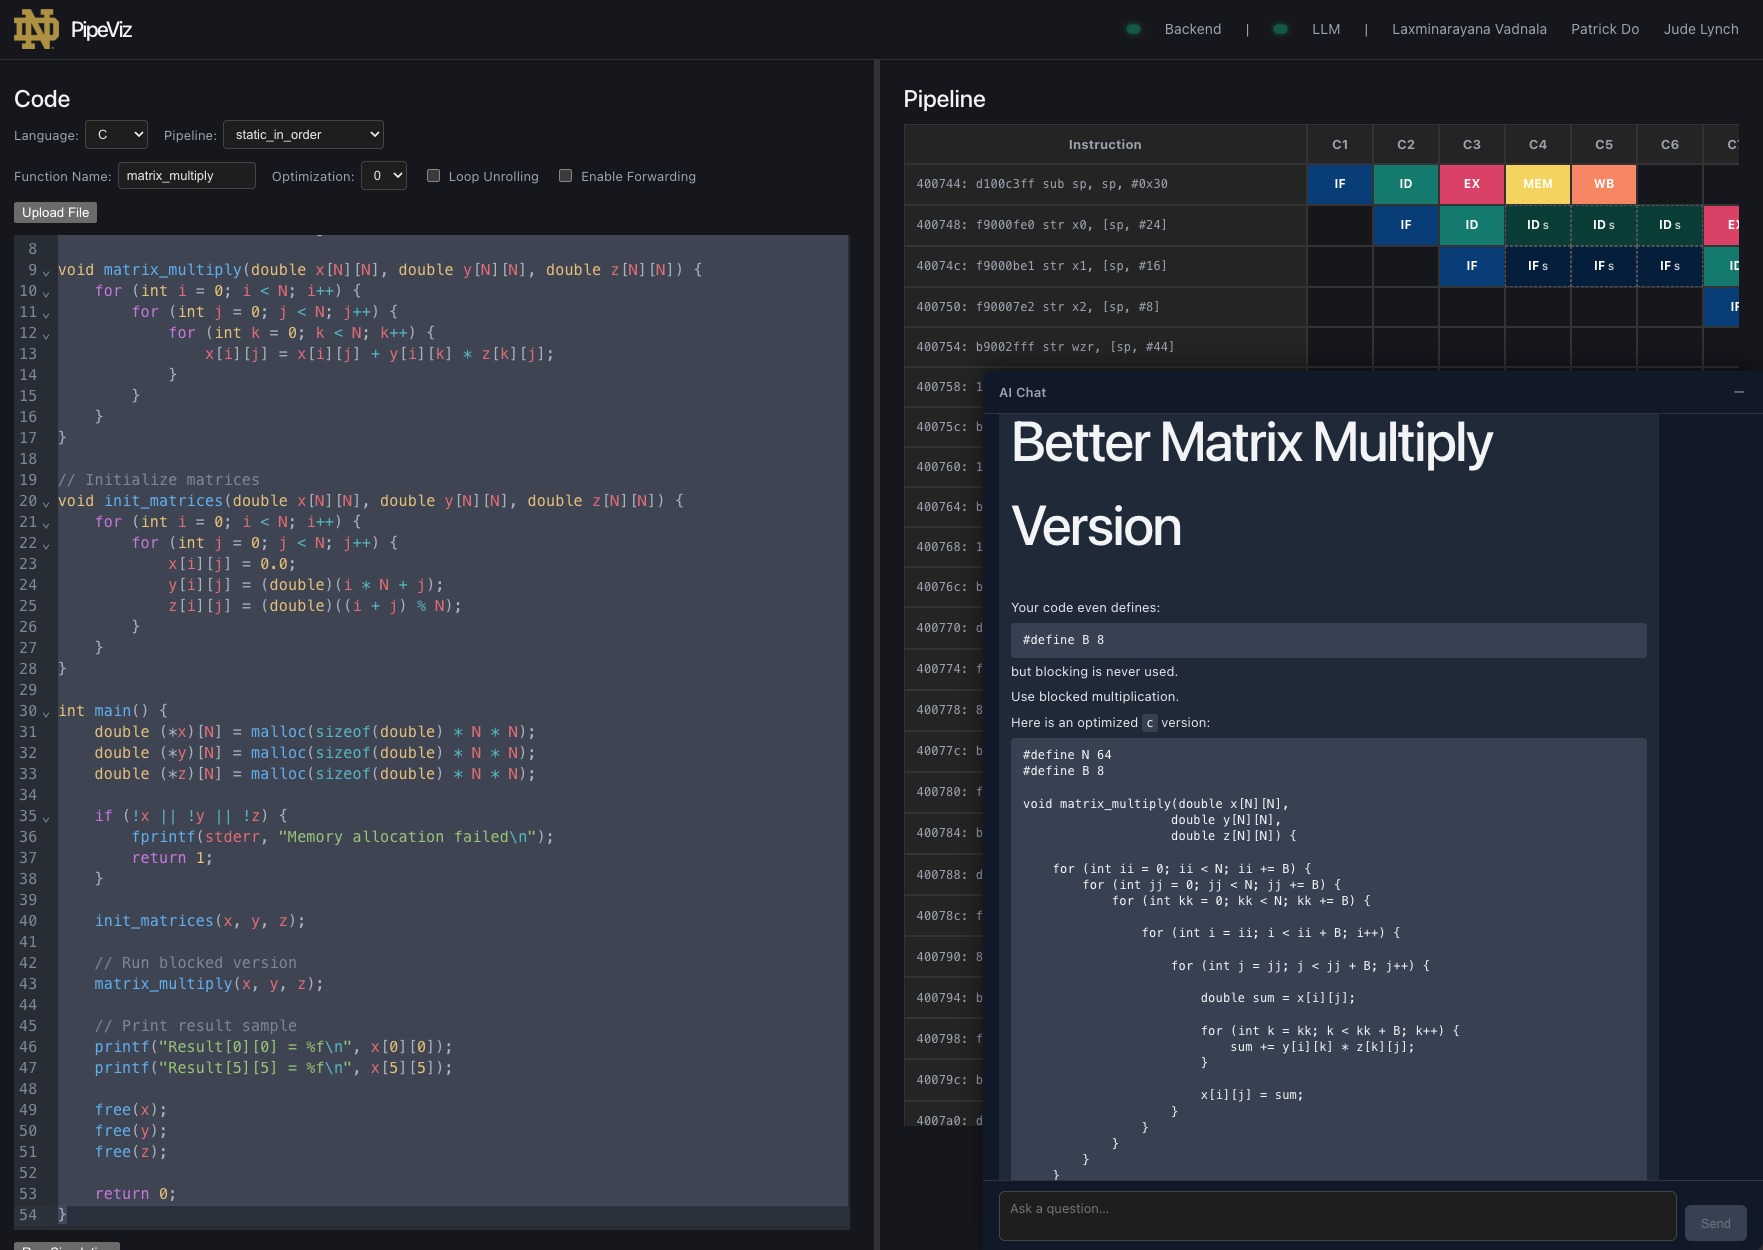
\includegraphics[width=\textwidth]{fig/LLM-matrix-multiply-response.png}
  \vspace{-0.25in}
  \caption{The PipeViz user interface showing the user code and optimal code suggested by the LLM based on the context fed to it while generating the response.}
  \label{fig:llm-matrix-response}
\end{figure*}

\textbf{Pipeline Simulation Analysis and Micro architectural Insights.} When both implementations were processed through identical pipeline configurations (static in-order, same compiler flags), the PipeViz tool revealed distinct hazard patterns and execution characteristics. The baseline implementation exhibited frequent \texttt{RAW} hazards in the innermost \texttt{k}-loop, where the load of \texttt{x[i][j]} for accumulation created dependencies with subsequent stores, forcing pipeline stalls in the \texttt{MEM} stage. The blocked version's use of a register-resident accumulator (\texttt{sum}) reduced these memory-dependent \texttt{RAW} hazards within each tile's inner loop, allowing more instruction-level parallelism despite the static in-order execution constraint. The visualization also highlighted differences in memory access patterns: the original code's column-major access to \texttt{z[k][j]} caused poor cache behavior visible as structural hazards on the memory unit, while the blocked version's smaller working set improved cache line utilization. The tool's ability to display these hazards alongside the assembly code enabled direct correlation between high-level algorithmic choices and low-level execution behavior. Here is the figure~\ref{fig:llm-matrix-response} shows the response from LLM

\textbf{Impact and Validation of LLM-Assisted Micro architectural Optimization.} This case study validates the efficacy of combining LLM code optimization with detailed pipeline simulation feedback. By providing the LLM with both the source code and the microarchitectural execution trace—including specific hazard locations and pipeline stall patterns—the system enabled context-aware optimization that addressed observable performance bottlenecks rather than applying generic transformations. The blocking optimization suggested by the LLM directly targeted the memory-hierarchy issues visible in the baseline pipeline simulation, demonstrating that language models can effectively reason about low-level performance when given appropriate micro-architectural context. This integrated approach creates a feedback loop where pipeline simulation informs optimization, and re-simulation validates improvements, providing developers with both actionable code changes and detailed visual evidence of their micro-architectural impact. The PipeViz tool thus serves not only as an educational platform for understanding pipeline behavior but as a practical optimization assistant capable of bridging the gap between high-level algorithm design and hardware execution reality.


\subsection*{Case Study 2. Loop-Unrolling Case Study in PipeViz}

% For the loop-unrolling case study, we used the same simple nested-loop kernel in C, compiled to AArch64 under the static in order pipeline model, and then compared two runs: one compiled with the loop-unrolling option enabled (vectorized, long straight-line kernel) and one compiled without loop unrolling (shorter loop body that iterates more frequently). In both cases, PipeViz ingests the generated assembly, simulates the program cycle by cycle through the five-stage pipeline (IF–ID–EX–MEM–WB), and records all observed RAW, WAR, WAW, and structural hazards directly from the simulated trace.
% Here is the code we have used for the experiment.

% \begin{lstlisting}[language=C, basicstyle=\ttfamily\scriptsize, tabsize=2]
% #include <stdio.h>

% int main(void) {
%     int n = 1000;
%     int sum = 0;
%     for (int i = 0; i < n; i++) {
%         for (int j = 0; j < n; j++) {
%             sum += i + j;
%         }
%     }
%     printf("sum = %d\n", sum);
%     return 0;
% }
% \end{lstlisting}


% In the non-unrolled version, the inner loop body is relatively compact: each iteration executes a handful of vector ADD and MLA instructions and then branches back. The pipeline simulation shows a dense chain of RAW dependencies along the main accumulation register ("v30") and the temporary vector registers ("v26", "v25", "v31"). Because we model a simple static in-order pipeline with ideal forwarding, most of these RAW dependencies do not show up as explicit stall cycles, but they still constrain the schedule: many instructions consume values that are produced only one or two cycles earlier, leaving very little slack. As a result, the pipeline has limited opportunity to overlap independent work. At the tail of the function, we also see a visible RAW stall between the horizontal reduction ("addv s31, v30.4s" or "addv s29, v1.4s") and the scalar move ("fmov w1, s31/s29"), which forces the ID stage of "fmov" to wait one cycle until the reduction result is written back. Finally, there is a structural hazard on the call to "printf": the branch-and-link ("bl") occupies the fetch path and produces an "IF[STALL]" in the next cycle while the pipeline redirects control flow.

%  In the unrolled configuration, the compiler expands the inner computation into a much longer straight-line vector kernel. We now see a wide strip of ADD and MLA operations over many different vector registers ("v17", "v19", "v20", "v21", "v22", "v23", "v24", "v25", "v26", "v30", "v31", etc.), rather than repeatedly executing a very short body. PipeViz’s hazard analysis shows that this transformation reduces the effective density of RAW hazards in the core loop: there are still true dependencies, but more of them are spread across independent accumulators instead of being tightly chained on a single register every few cycles. Because the static in-order model can now interleave independent vector operations, many potential RAW conflicts are naturally overlapped in EX, so we do not introduce additional stall cycles in the loop body. In other words, after loop unrolling, we are able to lower the number of stall-inducing RAW hazards in the hot loop, even though the total number of dynamic arithmetic instructions increases.


% The "-O2" compilation (first assembly) executes a compact loop that increments the counter by 1 (add w0, w0, \#0x1 at offset 0x56c) and performs minimal vector operations per iteration, creating a tight 20-byte loop body that branches back frequently. In contrast, the -O2 -funroll-loops version (second assembly) unrolls the loop to increment the counter by 10 (add w0, w0, \#0xa at offset 0x56c), expanding the loop body to ~208 bytes with multiple vector operations (movi, add, mla, mov instructions on vector registers v1-v31) that handle 10 loop iterations worth of computation in each iteration. This trade-off reduces branch prediction pressure and loop overhead—the branch penalty is paid only once per 10 iterations instead of per iteration—but at the cost of increased code size (0x148 bytes vs 0x74 bytes for main) and higher instruction-level parallelism demands. The unrolled version allows the CPU to exploit more parallelism across multiple independent vector operations within a single iteration, reducing data dependency stalls typical of tight loops, making it ideal for demonstrating how compiler optimizations interact with pipeline architecture in your project evaluation.

% Crucially, loop unrolling does not change the structural side of the pipeline in this experiment. In both the unrolled and non-unrolled traces, the only prominent structural event is still the call to "printf", which causes the same fetch-stage stall pattern around the "bl" instruction. The pipeline model still has a single branch back to the loop head and a single function call in the epilogue; unrolling modifies the amount of work done between branches, but it does not introduce or remove contended structural resources. As a result, the structural hazard profile remains essentially identical across the two runs: the same "IF[STALL]" at the call site and no new structural conflicts elsewhere.

% Finally, the end-of-loop reduction sequence behaves the same way in both configurations: the "addv" that collapses the vector accumulator into a scalar is immediately followed by "fmov" to move that scalar into a general-purpose register. In our static in-order model, this pair continues to manifest as a single RAW-induced stall at the ID stage of "fmov", regardless of whether the loop body was unrolled. The key impact of loop unrolling, therefore, is not to eliminate that final RAW hazard or to change structural hazards, but to reshape the inner-loop schedule so that more of the arithmetic is independent and can be overlapped, which shows up in PipeViz as fewer RAW-induced stalls in the hot region of the pipeline while leaving the structural hazard behavior effectively unchanged.

\textbf{Methodology and Experimental Setup.} This case study examines how the compiler optimization flag \texttt{-funroll-loops} affects pipeline execution behavior by comparing two compiled variants of the same nested-loop kernel. A simple double-nested summation program was submitted to the PipeViz pipeline visualization system under two configurations: a baseline compiled with \texttt{-O2} and an optimized variant compiled with \texttt{-O2 -funroll-loops}, both targeting AArch64 architecture. In each case, the generated assembly was simulated through the five-stage static in-order pipeline (IF$\rightarrow$ID$\rightarrow$EX$\rightarrow$MEM$\rightarrow$WB), with PipeViz automatically identifying and recording all RAW, WAR, WAW, and structural hazards at each clock cycle. The baseline simulation established a reference point for hazard frequency, stall patterns, and instruction scheduling behavior against which the unrolled variant could be directly compared. Here is the C source code used for the experiment:

\begin{lstlisting}[language=C, basicstyle=\ttfamily\scriptsize, tabsize=2]
#include <stdio.h>

int main(void) {
    int n = 1000;
    int sum = 0;
    for (int i = 0; i < n; i++) {
        for (int j = 0; j < n; j++) {
            sum += i + j;
        }
    }
    printf("sum = %d\n", sum);
    return 0;
}
\end{lstlisting}

\textbf{Compiler Loop Unrolling Strategy.} The \texttt{-funroll-loops} flag instructs the compiler to expand the inner loop body so that multiple iterations of computation are performed per loop cycle. In the baseline \texttt{-O2} compilation, the inner loop body is compact---approximately 0x74 bytes for \texttt{main}---incrementing the loop counter by one (\texttt{add w0, w0, \#0x1}) and branching back every iteration. The unrolled variant expands this into a substantially longer straight-line kernel of approximately 0x148 bytes, incrementing the counter by ten (\texttt{add w0, w0, \#0xa}) per iteration and computing ten iterations worth of work in a single pass using multiple vector registers (\texttt{v1}--\texttt{v31}) with interleaved \texttt{movi}, \texttt{add}, \texttt{mla}, and \texttt{mov} instructions. This transformation directly reduces branch prediction pressure and loop control overhead---the branch penalty is paid once per ten iterations rather than once per iteration---at the cost of increased code size and greater demands on instruction-level parallelism. By spreading accumulation across independent vector registers rather than repeatedly updating a single accumulator, the unrolled variant exposes more opportunities for the pipeline to overlap independent arithmetic operations.

\textbf{Pipeline Simulation Analysis and Micro architectural Insights.} When both variants were processed through the identical five-stage pipeline configuration, PipeViz revealed distinct hazard profiles that correspond directly to the structural differences introduced by loop unrolling. In the non-unrolled version, the inner loop body contains a dense chain of RAW dependencies concentrated on the primary accumulation register (\texttt{v30}) and associated temporary registers (\texttt{v25}, \texttt{v26}, \texttt{v31}). Although the static in-order model with ideal forwarding suppresses explicit stall cycles for most of these dependencies, the tight producer-consumer spacing leaves minimal scheduling slack and limits the pipeline's ability to overlap independent work. A visible RAW-induced stall does materialize at the loop epilogue: the horizontal reduction instruction (\texttt{addv s31, v30.4s}) is immediately followed by a scalar move (\texttt{fmov w1, s31}), forcing the ID stage of \texttt{fmov} to wait one cycle until the reduction result is written back. Additionally, the call to \texttt{printf} introduces a structural hazard that manifests as an \texttt{IF[STALL]} in the fetch stage while the pipeline redirects control flow after the branch-and-link instruction. In the unrolled configuration, PipeViz's hazard analysis shows that spreading accumulation across many independent vector registers materially reduces the effective density of stall-inducing RAW hazards within the hot loop body. Independent \texttt{ADD} and \texttt{MLA} operations on separate accumulators can be overlapped in the EX stage without incurring additional stalls, which is directly visible in the simulation trace as fewer hazard annotations in the core loop region. The structural hazard at the \texttt{printf} call site and the \texttt{addv}$\rightarrow$\texttt{fmov} RAW stall in the epilogue remain unchanged across both variants, confirming that loop unrolling modifies the inner-loop schedule without affecting the pipeline's behavior at function-call boundaries or scalar reduction sequences.

\textbf{Impact and Validation of Compiler-Driven Pipeline Optimization.} This case study validates PipeViz as a tool for directly observing the micro architectural consequences of compiler transformations. The key impact of loop unrolling is not the elimination of structural hazards or the final scalar reduction stall---both of which persist identically in both variants---but rather the reshaping of the inner-loop instruction schedule so that more arithmetic is independent and can be overlapped in execution. This improvement is visible in the PipeViz simulation trace as a reduction in RAW-induced stall annotations within the hot loop region, even as the total dynamic instruction count increases. The experiment also demonstrates a nuance that is difficult to observe without cycle-accurate simulation: loop unrolling's performance benefit is localized to the loop body itself, and code regions with inherently sequential data flow (such as the horizontal vector reduction followed by a scalar move) remain bottlenecks regardless of how aggressively the surrounding loop is transformed. PipeViz thus provides developers and students with precise, cycle-level evidence of where compiler optimizations create headroom and where fundamental data dependencies bound performance, bridging the gap between compiler optimization flags and their concrete effect on processor execution.